\documentclass[fontsize=11pt]{scrartcl}
%-------------------------------------------------------------------------------------------------
% LATEX TEMPLATE FOR A BACHELOR'S THESIS AT GHENT UNIVERSITY GLOBAL CAMPUS
% CREATED BY MANVEL GASPARYAN
% APRIL, 2021
%-------------------------------------------------------------------------------------------------
\usepackage{hyperref, tikz, float, subfigure, multicol, amsmath, amsthm, alphalph, amsfonts, amssymb, geometry, enumitem, parskip, xcolor, sectsty}
\usepackage[normalem]{ulem}
\usepackage[font=scriptsize,labelfont=bf]{caption}
\usepackage[explicit]{titlesec}
\usepackage[scaled]{helvet}
\renewcommand\familydefault{\sfdefault} 
\usepackage[T1]{fontenc}

\usepackage{setspace}

\usepackage{{listings}}

%-------------------------------------------------------------------------------------------------
 \geometry{a4paper, total={170mm,257mm}, left=20mm, right=20mm, top=25mm, bottom=30mm}
%-------------------------------------------------------------------------------------------------
\newtheorem{proposition}{Proposition}[section]
\newtheorem{lemma}{Lemma}[section]
\newtheorem{remark}{Remark}[section]
\newtheorem{corollary}{Corollary}[section]
\newtheorem{definition}{Definition}[section]
%-------------------------------------------------------------------------------------------------
\pagenumbering{roman}
\usepackage{fancyhdr}
\pagestyle{fancy}
\fancyhf{}
\renewcommand{\headrulewidth}{0pt}
\rhead{}
\lhead{}
\rfoot{\thepage}
\lfoot{}

%-------------------------------------------------------------------------------------------------
\definecolor{ghent_blue}{rgb}{0.1176, 0.392, 0.7843}
\definecolor{ghent_dark}{rgb}{0.0, 0.2, 0.4}
%-------------------------------------------------------------------------------------------------
\title{{\color{ghent_blue} TITLE: LATEX TEMPLATE FOR A BACHELOR'S THESIS AT GHENT UNIVERSITY GLOBAL CAMPUS}}
\subtitle{{\color{ghent_dark} [DOCUMENT SUBTITLE]}}
\date{}         
%-------------------------------------------------------------------------------------------------
\sectionfont{\fontsize{16}{15}\selectfont}
\sectionfont{\color{ghent_blue}}
%=================================================================================================
\begin{document}
%=================================================================================================
%PAGE i: TITLE PAGE 1
%-------------------------------------------------------------------------------------------------
\thispagestyle{empty}
\hfill
\includegraphics[scale = 1]{img/badge/2021.png}\\
%-------------------------------------------------------------------------------------------------
\vspace{8cm}

\noindent{\fontsize{30}{50}\selectfont{\color{ghent_blue}\noindent \hspace{12mm}\textbf{
Microphotonics %TITLE
}}}\\
\fontsize{20}{50}\selectfont{\color{ghent_dark}\noindent \hspace{13mm}\textbf{
CAD-LAB: Periodic Structure%SUBTITLE
}}\vspace{10mm}

\hspace{10mm}{\fontsize{10}{10}\selectfont{\textbf{
Lukuan Zhang, Rui Zhu, Xiyuan Guo%AUTHOR
}}}
\vspace*{\fill}
%-------------------------------------------------------------------------------------------------
\begin{flushleft}
\begin{figure}[b!]

\includegraphics[scale = 1.4]{img/badge/GUGC.pdf}
\end{figure}
\end{flushleft}

\doublespacing
\tableofcontents
\pagebreak
\pagenumbering{arabic}
%=================================================================================================
%HELP
%-------------------------------------------------------------------------------------------------
\section*{*  \uline{HELP}}
Once have been refered you can delete this part.\\
If you want to write an inline equation, code like this $E=mc^2$.\\
If you want to write a displayed equation without numbering, code like this $$E=mc^2$$\\
If you want to write a numbering displayed equation, code like this
\begin{equation} 
    E=mc^2 \label{eq1}
\end{equation}
and you can quote the equation by using Eq.\ref {eq1}.\\
\textbf{Tips:} The software \verb|Mathpix| can convert images and PDFs to LaTeX format which is
highly recommended by me.\\
List items like this:
\begin{enumerate} % itemize/description
    \item contents
    \item contents
\end{enumerate}
If you want to add one or more images as Figure \ref{name1} shown, you can copy the
code as following.\\
\begin{figure}[H]
    \centering
     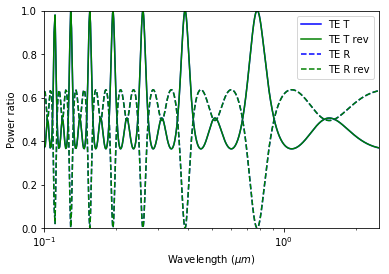
\includegraphics[width=0.35\textwidth]{img/1.png} % set width to get a proper ratio
     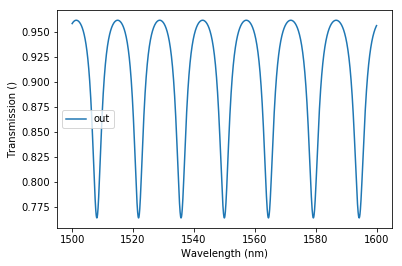
\includegraphics[width=0.35\textwidth]{img/2.png}
     \caption{Here to write the caption of the figure.}
     \label{name1}
\end{figure}
{\color{ghent_blue}Some details to notice:}
\begin{enumerate}
    \item  \textbf{Function name} and \textbf{units} should be presented in the Roman Regular Font.
    We can do this by using the sign backslash such as $\log(x)$, $\sin(x)$, $\cos(x)$, etc.
    \item When writing source codes in \LaTeX, make sure that the one-line code length 
    \textbf{does not} exceed one page(or 1/2 screen width on computer). Too long in width makes 
    a worse reading experience.
    \item Everytime when the new task comes, you are allowed to copy the whole template file and 
    rename it into the task name, then modify on the copy. Please don't modify the code directly
    on the template.
    \item Don't forget enter a space after the punstuation marks.
\end{enumerate}



%=================================================================================================
\pagebreak
%=================================================================================================
%TASK 1
\section{\uline{Distributed Bragg Refector}}
%-------------------------------------------------------------------------------------------------
%-------------------------------------------------------------------------------------------------
% Here comes some text. This text makes use of 1.5 line spacing. 
%-------------------------------------------------------------------------------------------------
\subsection{}
%-------------------------------------------------------------------------------------------------
From Figure \ref{fig1.1} of the $k$-vector diagram of the surface grating, 
the period of surface grating is calculated as $0.917\mathrm{\mu m}$.
\begin{figure}[H]
    \centering
     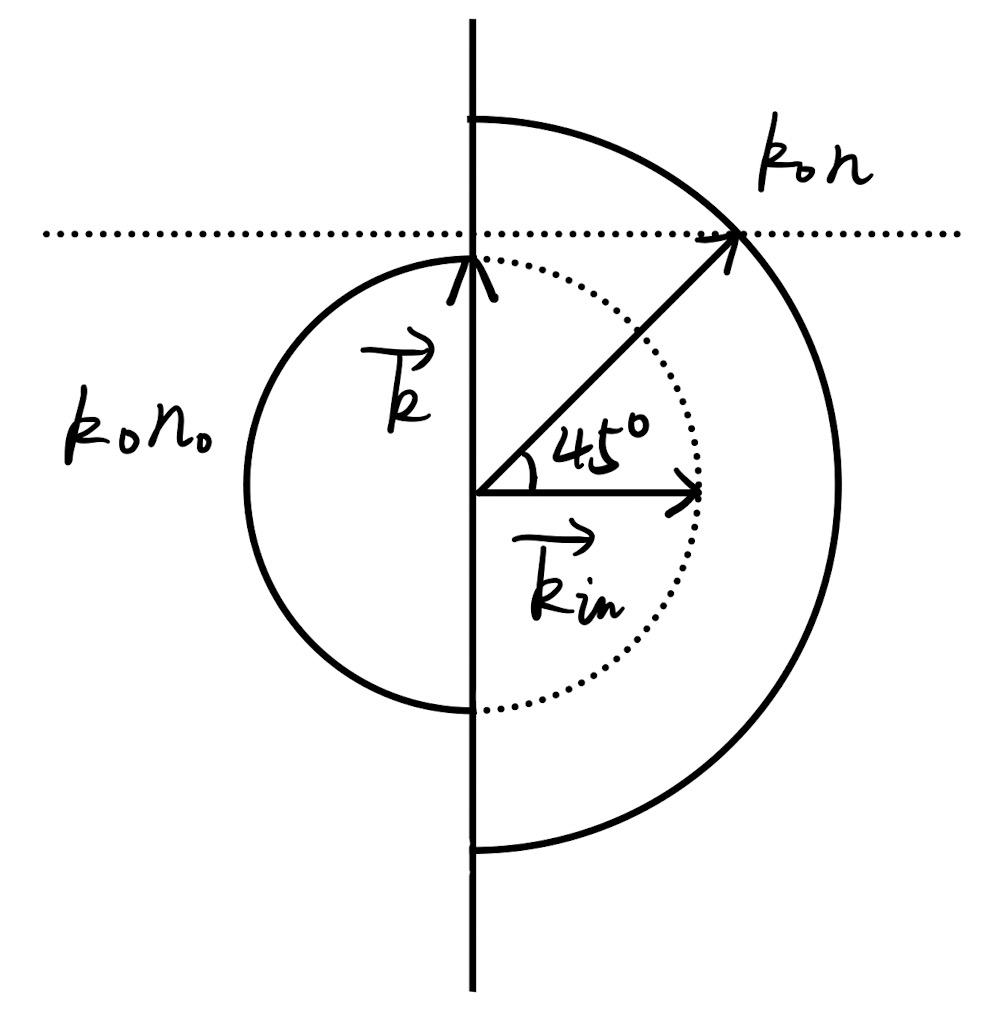
\includegraphics[width=0.6\textwidth]{img/fig1.1.png}
     \caption{The $k$-vector diagram of the surface grating}
     \label{fig1.1}
\end{figure}
%-------------------------------------------------------------------------------------------------
\subsection{}
%-------------------------------------------------------------------------------------------------
Set $D$ as $0.1\mathrm{\mu m}$ and period $\Lambda$ to $0.917\mathrm{\mu m}$ and 
run the simulation, then we can get figure \ref{fig1.2}, 
which shows the plane wave mainly propagates in the $0°$ direction, 
and partly propagates in the $45°$ and $-45°$ direction.
\begin{figure}[H]
    \centering
     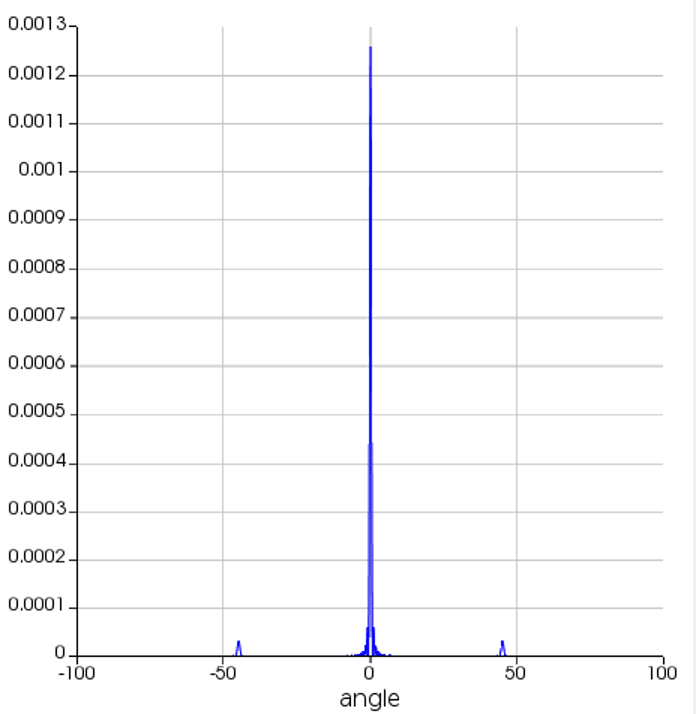
\includegraphics[width=0.45\textwidth]{img/fig1.2.png}
     \caption{Distribution of E2 in farfield with 
     period $0.917\mathrm{\mu m}$ and $D$ $0.1\mathrm{\mu m}$}
     \label{fig1.2}
\end{figure}
%-------------------------------------------------------------------------------------------------
\subsection{}
%-------------------------------------------------------------------------------------------------
\textbf{1. Increase the diffraction to the 45° orders}


%=================================================================================================
\pagebreak
%=================================================================================================
%TASK 2
%-------------------------------------------------------------------------------------------------
\section{\uline{Surface Grating}}
%-------------------------------------------------------------------------------------------------
Here comes some text. This text makes use of 1.5 line spacing. 
%-------------------------------------------------------------------------------------------------
\subsection{SUB-CHAPTER}
%-------------------------------------------------------------------------------------------------
Here comes some text. This text makes use of 1.5 line spacing. 
%-------------------------------------------------------------------------------------------------
\subsection{SUB-CHAPTER}
%-------------------------------------------------------------------------------------------------
Here comes some text. This text makes use of 1.5 line spacing. 
%-------------------------------------------------------------------------------------------------
\subsection{SUB-CHAPTER}
%-------------------------------------------------------------------------------------------------
Here comes some text. This text makes use of 1.5 line spacing. 
%=================================================================================================
\pagebreak
%=================================================================================================
%TASK 3
%-------------------------------------------------------------------------------------------------
\section{\uline{TASK 3}}
%-------------------------------------------------------------------------------------------------
Here comes some text. This text makes use of 1.5 line spacing. 
%-------------------------------------------------------------------------------------------------
\subsection{SUB-CHAPTER}
%-------------------------------------------------------------------------------------------------
Here comes some text. This text makes use of 1.5 line spacing. 
%-------------------------------------------------------------------------------------------------
\subsection{SUB-CHAPTER}
%-------------------------------------------------------------------------------------------------
Here comes some text. This text makes use of 1.5 line spacing. 
%-------------------------------------------------------------------------------------------------
\subsection{SUB-CHAPTER}
%-------------------------------------------------------------------------------------------------
Here comes some text. This text makes use of 1.5 line spacing. 
%=================================================================================================
\pagebreak
%=================================================================================================
%TASK 4
%-------------------------------------------------------------------------------------------------
\section{\uline{TASK 4}}
%-------------------------------------------------------------------------------------------------
Here comes some text. This text makes use of 1.5 line spacing. 
%-------------------------------------------------------------------------------------------------
\subsection{SUB-CHAPTER}
%-------------------------------------------------------------------------------------------------
Here comes some text. This text makes use of 1.5 line spacing. 
%-------------------------------------------------------------------------------------------------
\subsection{SUB-CHAPTER}
%-------------------------------------------------------------------------------------------------
Here comes some text. This text makes use of 1.5 line spacing. 
%-------------------------------------------------------------------------------------------------
\subsection{SUB-CHAPTER}
%-------------------------------------------------------------------------------------------------
Here comes some text. This text makes use of 1.5 line spacing. 
%=================================================================================================
\pagebreak
%=================================================================================================
%CTASK 5
%-------------------------------------------------------------------------------------------------
\section{\uline{TASK 5}}
%-------------------------------------------------------------------------------------------------
Here comes some text. This text makes use of 1.5 line spacing. 
%-------------------------------------------------------------------------------------------------
\subsection{SUB-CHAPTER}
%-------------------------------------------------------------------------------------------------
Here comes some text. This text makes use of 1.5 line spacing. 
%-------------------------------------------------------------------------------------------------
\subsection{SUB-CHAPTER}
%-------------------------------------------------------------------------------------------------
Here comes some text. This text makes use of 1.5 line spacing. 
%-------------------------------------------------------------------------------------------------
\subsection{SUB-CHAPTER}
%-------------------------------------------------------------------------------------------------
Here comes some text. This text makes use of 1.5 line spacing. 
%=================================================================================================
\pagebreak
%=================================================================================================
%TASK 6
%-------------------------------------------------------------------------------------------------
\section{\uline{TASK 6}}
%-------------------------------------------------------------------------------------------------
Here comes some text. This text makes use of 1.5 line spacing. 
%-------------------------------------------------------------------------------------------------
\subsection{SUB-CHAPTER}
%-------------------------------------------------------------------------------------------------
Here comes some text. This text makes use of 1.5 line spacing. 
%-------------------------------------------------------------------------------------------------
\subsection{SUB-CHAPTER}
%-------------------------------------------------------------------------------------------------
Here comes some text. This text makes use of 1.5 line spacing. 
%-------------------------------------------------------------------------------------------------
\subsection{SUB-CHAPTER}
%-------------------------------------------------------------------------------------------------
Here comes some text. This text makes use of 1.5 line spacing.  %=================================================================================================
\pagebreak
%=================================================================================================
%Appendix A
%-------------------------------------------------------------------------------------------------
% \section*{\uline{APPENDIX A}}
% %-------------------------------------------------------------------------------------------------
% Here comes some text. This text makes use of 1.5 line spacing. %=================================================================================================
% \pagebreak
%=================================================================================================
% %Appendix B
% %-------------------------------------------------------------------------------------------------
% \section*{\uline{APPENDIX B}}
% %-------------------------------------------------------------------------------------------------
% Here comes some text. This text makes use of 1.5 line spacing.\\
% In order to cite use \cite{Bern:1}, \cite{Bez:1}, \cite{BioModels}, \cite{Row:1} %=================================================================================================
% \pagebreak
% %=================================================================================================
% \bibliographystyle{plain}
% \bibliography{References}
%=================================================================================================

\end{document}